
% This LaTeX was auto-generated from an M-file by MATLAB.
% To make changes, update the M-file and republish this document.

\documentclass{article}
\usepackage{graphicx}
\usepackage{color}

\sloppy
\definecolor{lightgray}{gray}{0.5}
\setlength{\parindent}{0pt}

\begin{document}

    
    
\subsection*{Contents}

\begin{itemize}
\setlength{\itemsep}{-1ex}
   \item Problem 1
   \item Part 1
   \item Part 2
   \item Part 3
   \item Part 4
   \item Part 5
   \item Part 6
   \item Problem 2
   \item Part 1
   \item Part 2
   \item Part 3
   \item Part 4
   \item Part 5
   \item Part 6
   \item Part 7
   \item Part 8
   \item Problem 3
\end{itemize}
\begin{par}
Image preprocessing...
\end{par} \vspace{1em}
\begin{verbatim}
clear all;
clc;
close all;
%code for my custom functions can be found on
%https://github.com/curtismuntz/machine_vision/tree/master/commonFunctions
addpath ../commonFunctions
I = getIMG('Tux2.png');
I = imresize(I,[400,400]);
I = rgb2gray(I);
I = im2double(I);
imshow(I);
title('Original Image');
\end{verbatim}

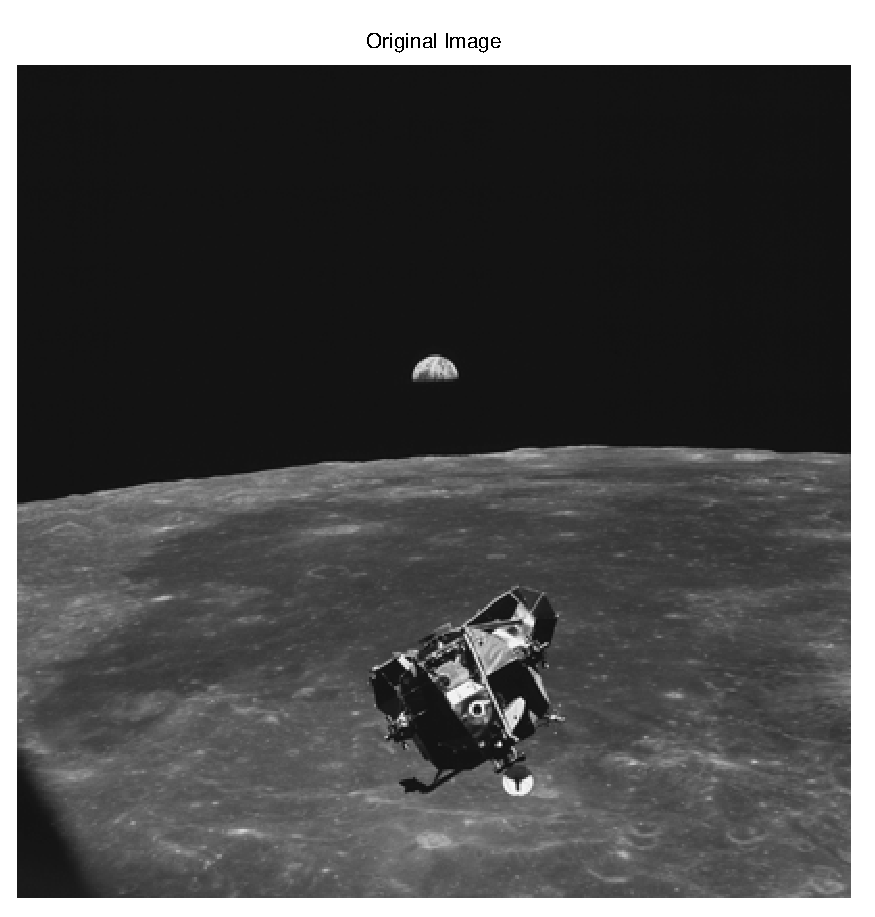
\includegraphics [width=4in]{hw4_01.eps}


\subsection*{Problem 1}

\begin{par}
Edge detection in the space domain.
\end{par} \vspace{1em}
\begin{par}
Pick an image with visible horizontal and vertical edges.
\end{par} \vspace{1em}


\subsection*{Part 1}

\begin{verbatim}
%Apply the horizontal Sobel mask to the image. Show the result.
figure('name', 'horizontal sobel mask')
sobelX=double([-1 0 1; -2 0 2; -1 0 1])
horiz = convolution(I, sobelX);
imshow(im2uint8(horiz));
title('SobelX Masked Image')
\end{verbatim}

        \color{lightgray} \begin{verbatim}
sobelX =

    -1     0     1
    -2     0     2
    -1     0     1

\end{verbatim} \color{black}
    
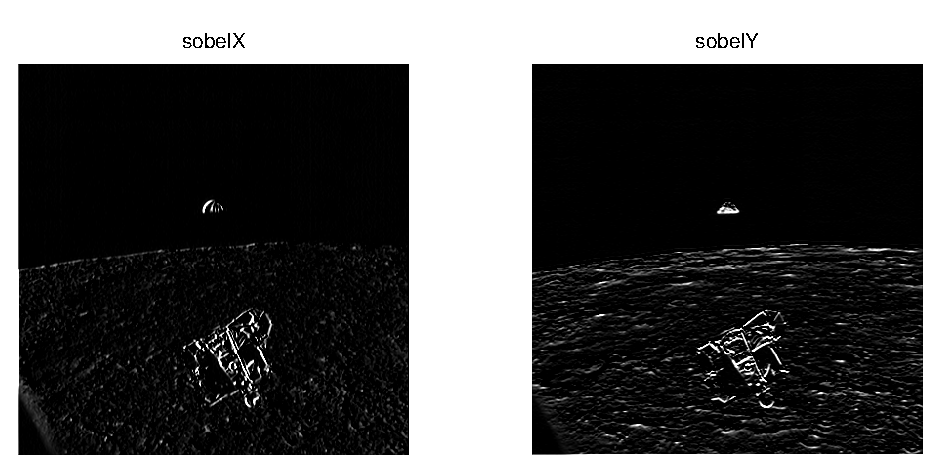
\includegraphics [width=4in]{hw4_02.eps}


\subsection*{Part 2}

\begin{verbatim}
%Apply the vertical Sobel mask to the image. Show the result and compare
%with the previous question. Discuss your results.
figure('name', 'vertical sobel mask')
sobelY=double([1 2 1; 0 0 0; -1 -2 -1])
vert = convolution(I, sobelY);
imshow(im2uint8(vert));
title('SobelY Masked Image')
\end{verbatim}

        \color{lightgray} \begin{verbatim}
sobelY =

     1     2     1
     0     0     0
    -1    -2    -1

\end{verbatim} \color{black}
    
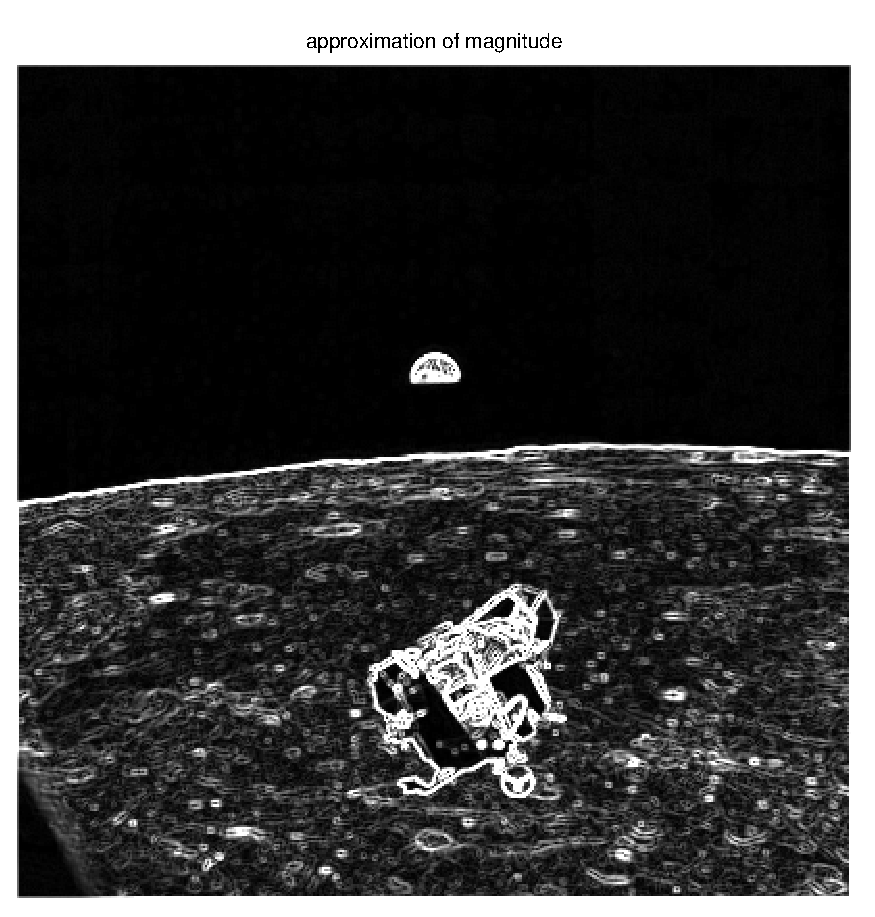
\includegraphics [width=4in]{hw4_03.eps}
\begin{par}
The horizontal sobel mask is detecting the vertical edges, and the vertical sobel mask is detecting the horizontal edges. There seems to be a little bit of crossover between the two (vertical is detecting a vertical edge, and vice versa).
\end{par} \vspace{1em}


\subsection*{Part 3}

\begin{verbatim}
%Use the magnitude to combine horizontal and vertical edges. Show the result.
figure('name','magnitude'); %pop pop
magnitude = abs(horiz) + abs(vert);
imshow(magnitude);
title('Approximation of Magnitude');
\end{verbatim}

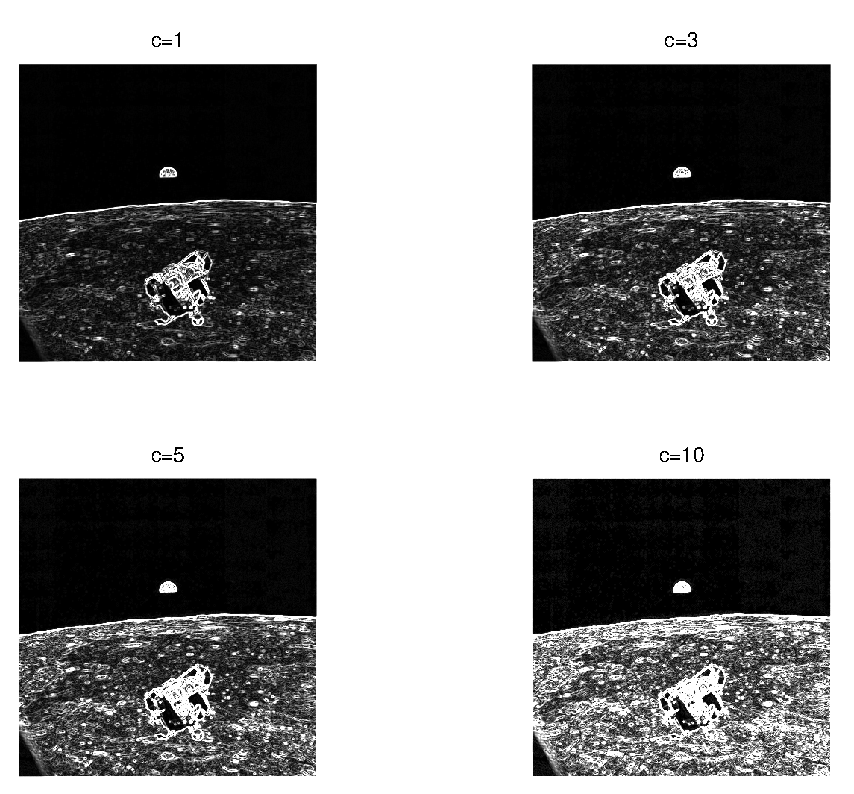
\includegraphics [width=4in]{hw4_04.eps}


\subsection*{Part 4}

\begin{verbatim}
%In the Sobel mask, the constant c = 2. We want to see the effect of c on the
%edge detection process, try different values and see what happens.
figure('name', 'Using Various Values for c in Sobel Mask')
subplot(221)
c=1;
sobelX=double([-1 0 1; -c 0 c; -1 0 1]);
sobelY=double([1 c 1; 0 0 0; -1 -c -1]);
h=convolution(I,sobelX);
v=convolution(I,sobelY);
C=(abs(h)+abs(v));
imshow(C);
title('c=1')

subplot(222);
c=3;
sobelX=double([-1 0 1; -c 0 c; -1 0 1]);
sobelY=double([1 c 1; 0 0 0; -1 -c -1]);
h=convolution(I,sobelX);
v=convolution(I,sobelY);
C=(abs(h)+abs(v));
imshow(C);
title('c=3')

subplot(223)
c=5;
sobelX=double([-1 0 1; -c 0 c; -1 0 1]);
sobelY=double([1 c 1; 0 0 0; -1 -c -1]);
h=convolution(I,sobelX);
v=convolution(I,sobelY);
C=(abs(h)+abs(v));
imshow(C);
title('c=5')


subplot(224)
c=10;
sobelX=double([-1 0 1; -c 0 c; -1 0 1]);
sobelY=double([1 c 1; 0 0 0; -1 -c -1]);
startS=tic; %asked for part 6
h=convolution(I,sobelX);
v=convolution(I,sobelY);
C=(abs(h)+abs(v));
sobeltime= toc(startS);
imshow(C);
title('c=10')
\end{verbatim}

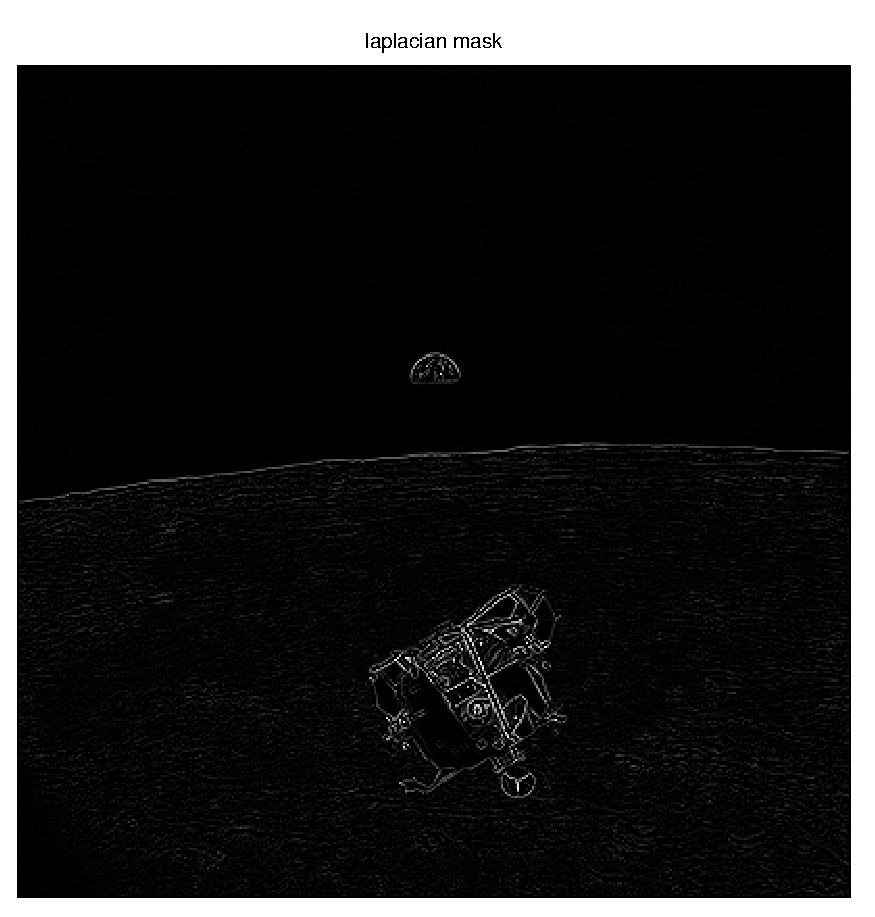
\includegraphics [width=4in]{hw4_05.eps}
\begin{par}
As the value for $c$ increases, the resultant convolution of the masks detect more parts of the image as edges.
\end{par} \vspace{1em}


\subsection*{Part 5}

\begin{verbatim}
%Use the Laplacian mask to perform edge detection on the same image.
%Compare with the results of question 3).
figure('name', 'laplacian mask')
L=[0 1 0; 1 -4 1; 0 1 0];
startL = tic;
laplacedI=convolution(I,L);
laplacetime = toc(startL);
imshow(im2uint8(laplacedI)), title('Laplacian Mask');
rmpath ../commonFunctions
\end{verbatim}

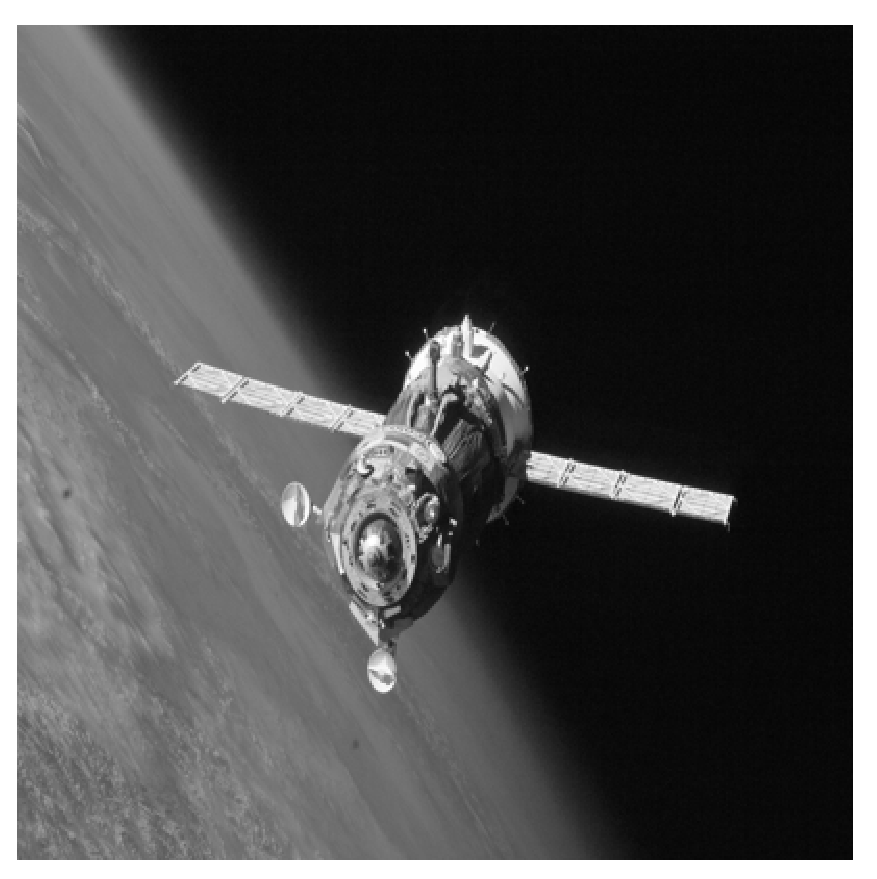
\includegraphics [width=4in]{hw4_06.eps}
\begin{par}
The laplacian mask seems to produce the same image as the magnitude of the Sobel masks did.
\end{par} \vspace{1em}


\subsection*{Part 6}

\begin{verbatim}
%Compare between the Laplacian and Sobel masks in terms of the computation
%time, use Matlab command tic - toc. For the Sobel mask, you need to
%consider the complete implementation, that is edge detection in both
%directions.

%-- these were calculated in parts 4 and 5 respectively
sprintf('sobel approach: %s',sobeltime)
sprintf('laplacian approach: %s', laplacetime)
\end{verbatim}

        \color{lightgray} \begin{verbatim}
ans =

sobel approach: 1.966261e-01


ans =

laplacian approach: 7.457914e-02

\end{verbatim} \color{black}
    \begin{par}
The sobel approach takes longer, primarily because the operation is applying two masks, whereas the Laplacian approach only applies one.
\end{par} \vspace{1em}


\subsection*{Problem 2}

\begin{par}
Edge detection in the frequency domain.
\end{par} \vspace{1em}


\subsection*{Part 1}

\begin{verbatim}
%Obtain the FFT of the horizontal and vertical Sobel masks.
%You need to perform zero padding.
addpath ../commonFunctions
%I2 = getIMG('Soyuz_TMA-19_spacecraft_departs_the_ISS.jpg');
I2 = getIMG('ed3.jpg');
rmpath ../commonFunctions
%I2 = im2double(rgb2gray(imresize(I2,[401,401])));
I2 = imresize(I2,[401,401]);
figure('name','Problem 2 Image');
imshow(I2);
title('Problem 2 Original Image');

figure('name','ffts of Sobel Masks');
c=2;
sobelX=double([-1 0 1; -c 0 c; -1 0 1]);
sobelY=double([1 c 1; 0 0 0; -1 -c -1]);
%work on making this more general..........
sobelX1 = padarray(sobelX,[199,199]);
sobelFFTX=fft2(sobelX1);
%work on making this more general..........
sobelY1 = padarray(sobelY,[199,199]);
sobelFFTY=fft2(sobelY1);

subplot(121), imshow(sobelFFTX), title('SobelX fft');
subplot(122), imshow(sobelFFTY), title('SobelY fft');
\end{verbatim}

        \color{lightgray} \begin{verbatim}Warning: Displaying real part of complex input. 
Warning: Displaying real part of complex input. 
\end{verbatim} \color{black}
    
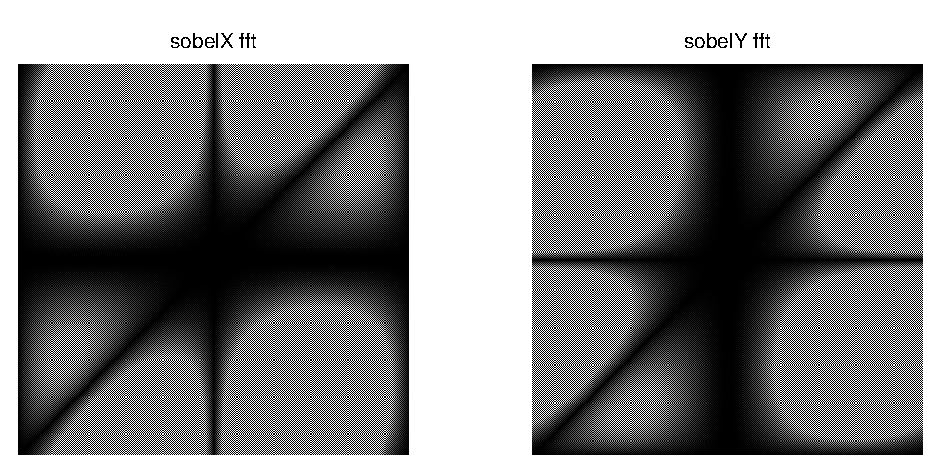
\includegraphics [width=4in]{hw4_07.eps}

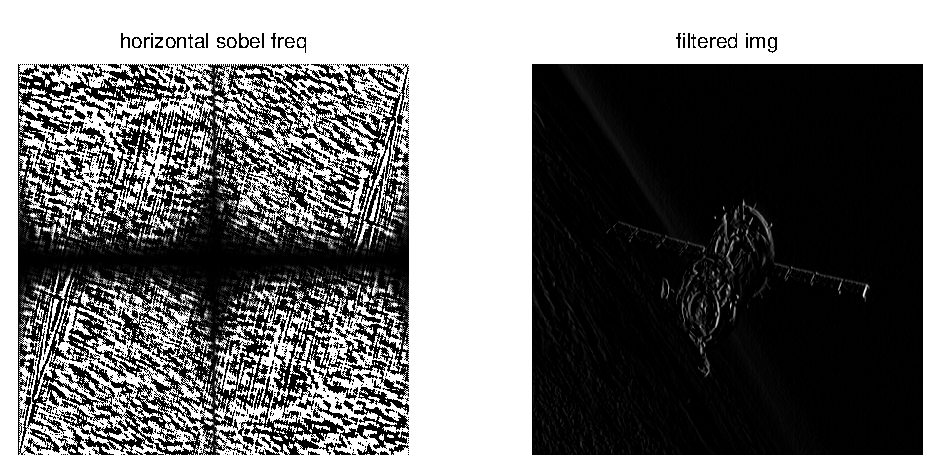
\includegraphics [width=4in]{hw4_08.eps}


\subsection*{Part 2}

\begin{verbatim}
%Perform filtering in the frequency domain using the horizontal Sobel mask.

figure('name', 'frequency horizontal filtering');
horizF=fft2(I2).*sobelFFTX;
horizS=ifft2(horizF);
dmin = min(min(abs(horizS)));
dmax = max(max(abs(horizS)));
subplot(121), imshow(horizF), title('Horizontal Sobel fft Mask');
subplot(122), imshow(ifftshift(horizS),[dmin dmax]), title('Filtered Image');
\end{verbatim}

        \color{lightgray} \begin{verbatim}Warning: Displaying real part of complex input. 
\end{verbatim} \color{black}
    
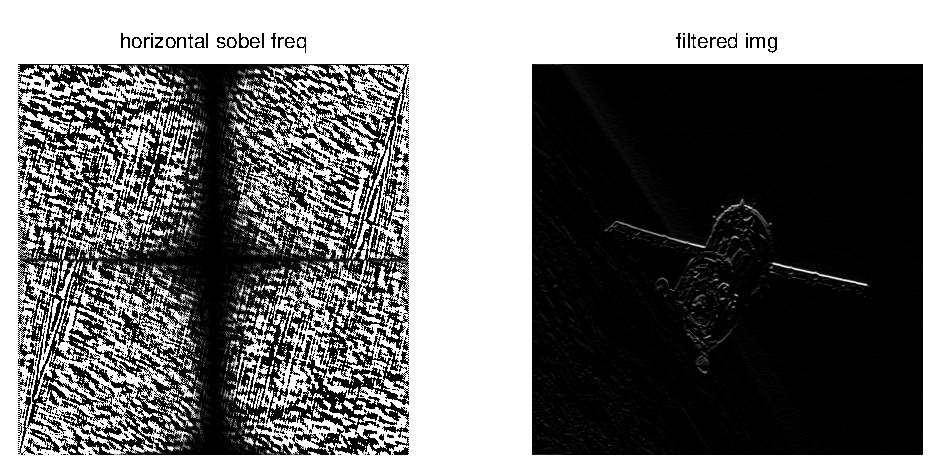
\includegraphics [width=4in]{hw4_09.eps}


\subsection*{Part 3}

\begin{verbatim}
%Perform filtering in the frequency domain using the vertical Sobel mask.
figure('name', 'frequency vertical filtering');
vertF=fft2(I2).*sobelFFTY;
vertS=ifft2(vertF);
dmin = min(min(abs(vertS)));
dmax = max(max(abs(vertS)));
subplot(121), imshow(vertF), title('Vertical Sobel fft Mask');
subplot(122), imshow(ifftshift(vertS),[dmin dmax]), title('Filtered Image');
\end{verbatim}

        \color{lightgray} \begin{verbatim}Warning: Displaying real part of complex input. 
\end{verbatim} \color{black}
    
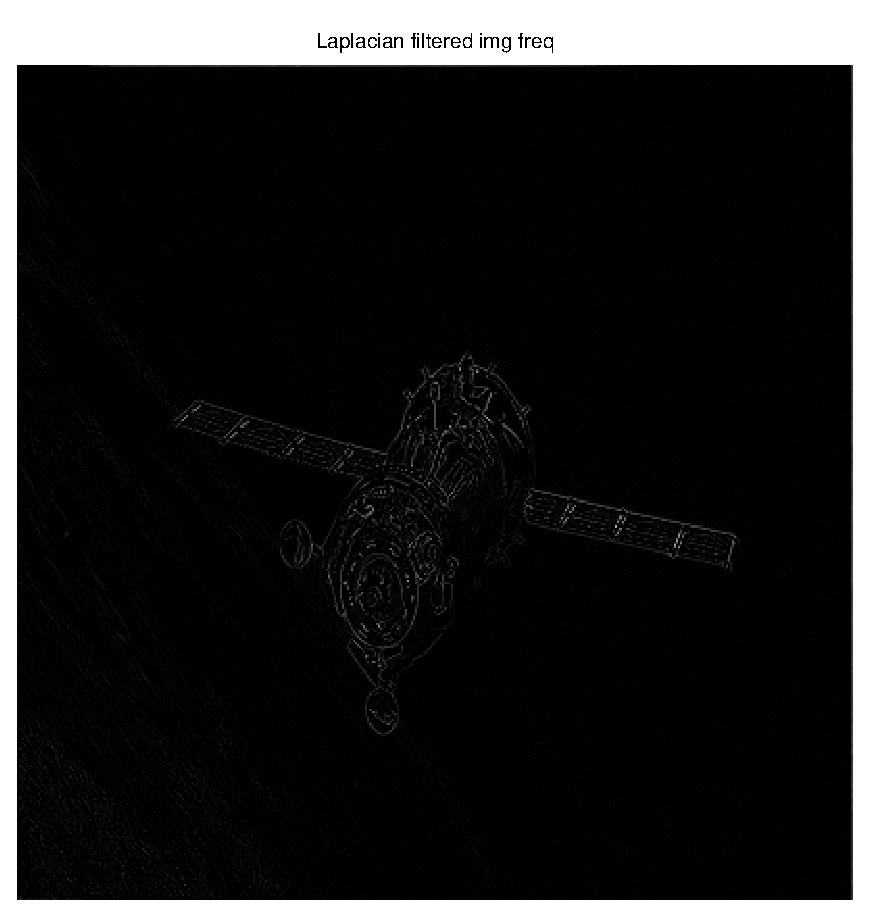
\includegraphics [width=4in]{hw4_10.eps}


\subsection*{Part 4}

\begin{verbatim}
%Obtain the FFT of the Laplacian mask. You need to perform zero padding.
L1 = fft2(padarray(L,[199,199]));
\end{verbatim}


\subsection*{Part 5}

\begin{verbatim}
%Perform filtering in the frequency domain using Laplacian to detect
%the edges.
figure('name','laplacian frequency filtering');
lapF=fft2(I2).*L1;
lapS=ifft2(lapF);
dmin = min(min(abs(lapS)));
dmax = max(max(abs(lapS)));
imshow(ifftshift(lapS),[dmin dmax]), title('Laplacian Filtered Image (Freq. domain)');
\end{verbatim}

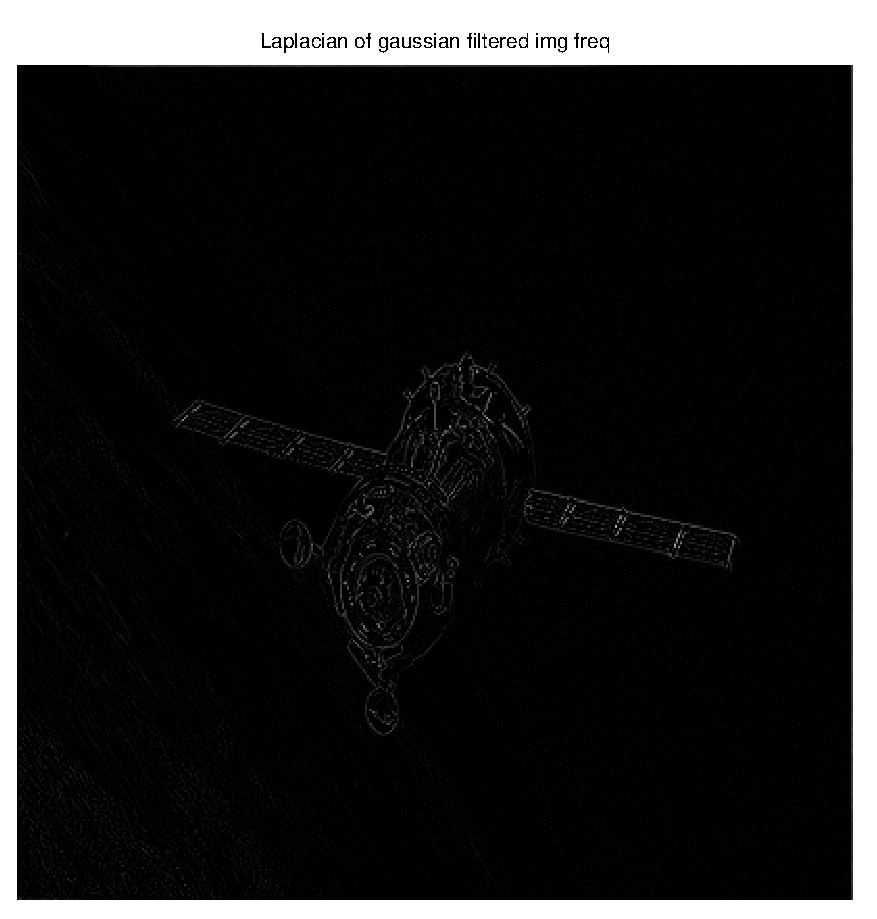
\includegraphics [width=4in]{hw4_11.eps}


\subsection*{Part 6}

\begin{verbatim}
%Construct a 3 by 3 mask for the Laplacian of Gaussian (LoG) and then obtain
%its FFT. You can use fspecial for this question.
%addpath ../commonFunctions
%gauss=gaussfilter(3, 1/2);
%LoG=L*gauss;
%LoGF=fft2(LoG);
%rmpath ../commonFunctions
LoG=fspecial('log',[401,401]);
LoGF=fft2(LoG);
\end{verbatim}


\subsection*{Part 7}

\begin{verbatim}
%Perform filtering in the frequency domain using LoG to detect the edges.
I3=fft2(I2).*L1;
lapS=ifft2(I3);
dmin = min(min(abs(lapS)));
dmax = max(max(abs(lapS)));
\end{verbatim}


\subsection*{Part 8}

\begin{verbatim}
%Show and discuss your results.
figure('name','laplacian of gaussian freq filtering');
imshow(ifftshift(lapS),[dmin dmax]);
title('Laplacian of gaussian filtered img freq');
\end{verbatim}

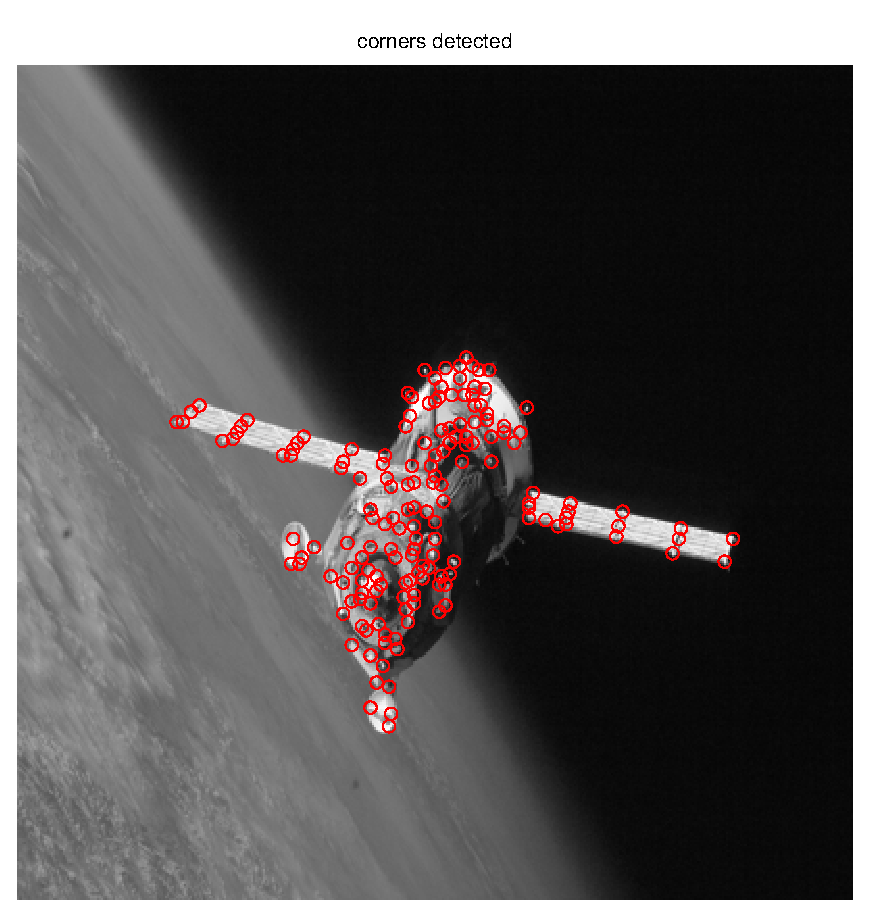
\includegraphics [width=4in]{hw4_12.eps}
\begin{par}
The FFT of the Laplacian of Gaussian is very effective at finding the edges in the image.
\end{par} \vspace{1em}


\subsection*{Problem 3}

\begin{par}
The Harris detector was introduced in 1988 for corner detection. An illustration is shown in figure 2. Apply the Harris detector to an image of your choice. Pick an image with visible corners. Mark all corners on the image in a similar way to figure 2 Do you think the Harris edge detector is a linear filtering operation? Explain
\end{par} \vspace{1em}
\begin{verbatim}
figure('name','corner detection');
C=corner(I2); %to find corner points
imshow(I2);hold on, plot(C(:,1),C(:,2),'ro')
title('corners detected')
\end{verbatim}

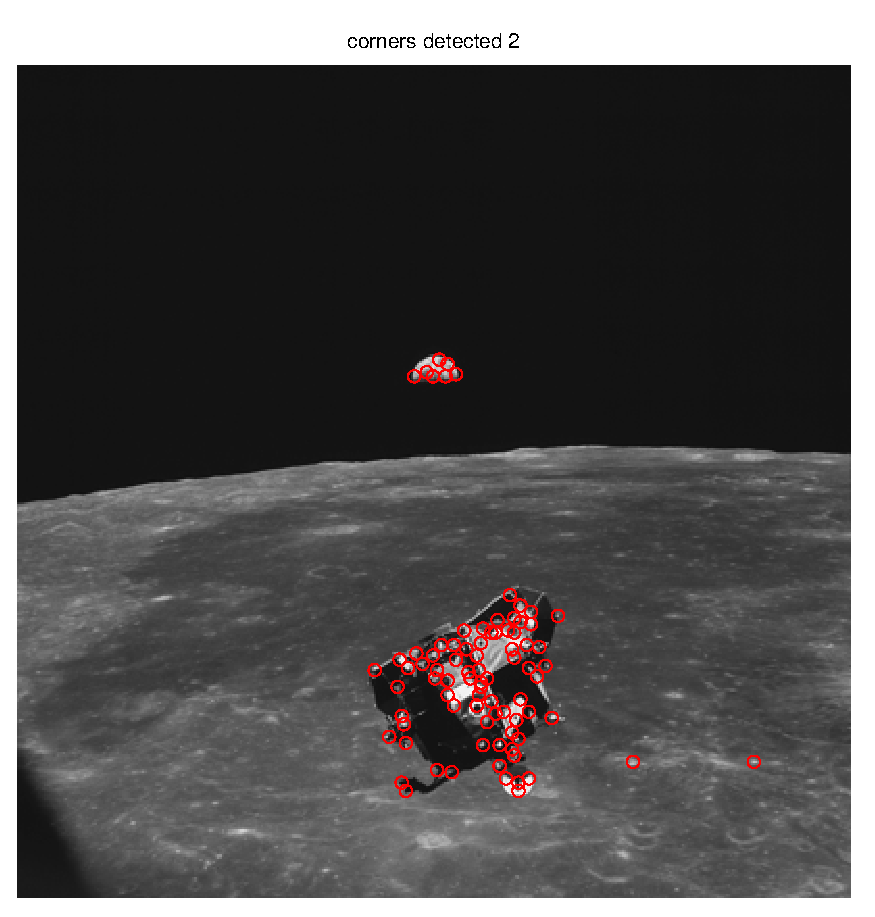
\includegraphics [width=4in]{hw4_13.eps}
\begin{par}
The built in corner detection funciton was able to pick up all the corners in the image. The funciton is not linear, as it calculates its mask based off of gradients within a range of the pixel values, and not use a mask on the pixel values.
\end{par} \vspace{1em}



\end{document}
    
